\documentclass{article}
\usepackage[utf8]{inputenc}
\usepackage{graphicx}
\usepackage{amsmath}
\usepackage{tipa}
\usepackage{amssymb}
\usepackage{algpseudocode}
\usepackage{tikz} 

\title{Tema1}
\author{Tiganus Ionel, Grigore Valerian, grupa A3}
\date{November 2022}

\begin{document}
\maketitle
\large
\section*{Exercitiul 1}

\quad a) Avem 2 cazuri extreme:

    \quad cazul minim: cand toate tramvaiele au statia \textit{i} in comun si intervalele de asteptare se suprapun \textit{((start\small{i}\large, end\small{i}\large) $\cap$ (start\small{j}\large, end\small{j}\large) $\neq$ $\emptyset$)}
    

    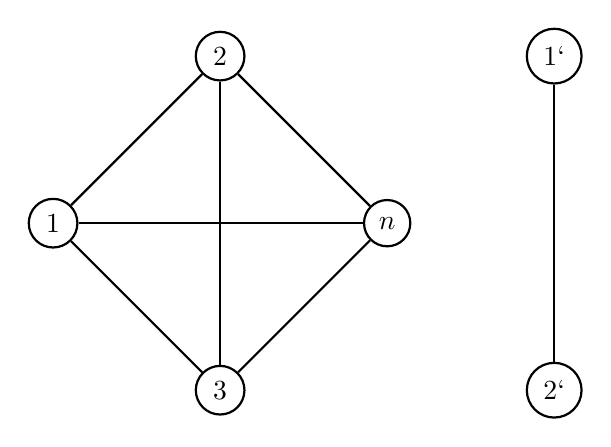
\begin{tikzpicture}[node distance={30mm}, thick, main/.style = {draw, circle}]
    \node[main] (1) {$1$};
    \node[main] (2) [above right of=1] {$2$};
    \node[main] (3) [below right of=1] {$3$}; 
    \node[main] (4) [above right of=3] {$n$};
    \node[main] (5) [above right of=4] {$1`$}; 
    \node[main] (6) [below right of=4] {$2`$};
    \draw (1) -- (2);
    \draw (1) -- (3);
    \draw (1) -- (4);
    \draw (2) -- (3);
    \draw (2) -- (4);
    \draw (3) -- (4);
    \draw (5) -- (6);
    \end{tikzpicture}
    
     In desenul alaturat prima componenta cu nodurile \textit{1,2,3,n} este reprezentata de tramvaiele \textit{1,2,3,...,n} care sunt in statia 1 iar cea dea doua componenta conexa este data de tramvaiele \textit{1`,2`} care sunt in statia \textit{n} (asta e o reprezentare minimala a cazului acestuia).
    
      Deci cazul minim cuprinde \textit{n} grupari (\textit{n} dat de cele \textit{n} statii) de cate \textit{m} tramvaie, adica \textit{n} componente conexe.
     
     \quad cazul maxim: cand toate tramvaiele au statia \textit{i} in comun si intervalele de asteptare nu se suprapun \textit{((start\small{i}\large, end\small{i}\large) $\cap$ (start\small{j}\large, end\small{j}\large) = $\emptyset$)}
     
    \begin{tikzpicture}[node distance={30mm}, thick, main/.style = {draw, circle}]
    \node[main] (1) {$1$};
    \node[main] (2) [above right of=1] {$2$};
    \node[main] (3) [below right of=1] {$3$}; 
    \node[main] (4) [above right of=3] {$n$};
    \node[main] (5) [above right of=4] {$1`$}; 
    \node[main] (6) [below right of=4] {$2`$};
    \end{tikzpicture}
    
       Deci cazul maxim cuprinde \textit{n*m} grupari, adica \textit{n*m} componente conexe.
    
      Deci numarul de componente conexe ale lui \textit{G} este cel putin numarul de statii de tramvai.
     
b) Conform teoriei: \textit{O submultime de k noduri a unui graf G care induce un graf complet este numita k-clica, numarul de clica al lui G este w(G) = max $\mid$Q$\mid$ unde Q este clica in G}].
    \newline
    \quad Daca ne uitam la enuntul problemei si la subpunctul \textit{a)} (mai ales cazul minim) observam ca tramvaiele cu statia comuna care se regasesc in acelasi timp sunt adiacente intre ele unde \textit{k} din definitie e data de numarul maxim de tramvaie si aceasta reprezinta \textit{w(G)}.  
     
c) Stim ca fiecare componenta conexa a grafului \textit{G} este un graf complet. Daca vom lua macar o componenta conexa cu cel putin 3 noduri din \textit{G} vom avea mereu un circuit indus de lungime 3 (fiecare graf complet are un circuit indus de 3 noduri) deci \textit{G} nu va avea circuit indus \textit{$\geq$4}.

d)
\begin{algorithmic}
\For{$(v \in V)$}
    \State $visitedNeighbors[v] \leftarrow 0;$
\EndFor
\State $Q \leftarrow 0;$
\For{$(v \in V)$}  
    \State $countV \leftarrow 0;$
    \State $S \leftarrow \emptyset;$
    \If {$(visitedNeighbors[v] = 0)$} 
        \State $countV \leftarrow 1;$
        \State $visitedNeighbors[v] \leftarrow 1;$
        \State $S \leftarrow S \cup \{v\};$
        \While {$(S \neq \emptyset)$}
            \State $v \leftarrow S[0]; //primul Element Din Coada$
            \State $m \leftarrow v;$
            \State $S \leftarrow S \backslash \{v\};$
            \For{$n \in N\tiny{G}\large(m)$}
                \If {$(visitedNeighbors[n] = 0)$}
                    \State $visitedNeighbors[n]\leftarrow 1;$
                    \State $countV \leftarrow countV + 1;$
                    \State $S \leftarrow S \cup \{n\};$
                \EndIf
            \EndFor
        \EndWhile
    \EndIf
    \State $Q \leftarrow max(countV,Q);$
\EndFor

Complexitatea algoritmului este de \textit{O(n + m)} data de algoritmul \textit{BFS} iar algoritmul functioneaza astfel: 
    
    -vede daca este deja vizitata componenta conexa 
    
    -daca nu este vizitata va lua nodul respectiv din lista de noduri si va lua toti vecinii acestuia (totodata in \textit{countV} se va aduna cu 1 de fiecare data cand dam de un vecin)
    
    -se va repeta procesul si cu vecinii vecinilor pana cand toata componenta conexa este deja vizitata (cand lista \textit{S} ramane vida)
    
    -cand trecem de la o componenta la alta numarul de noduri din componentele conexe se vor trece in \textit{Q} (in cazul in care este mai mare valoarea acesteia, evident)

Operatia \textit{O(1)} este data de \textit{countV} care va memora cate noduri avem in componenta conexa.

\end{algorithmic}

\section*{Exercitiul 2}
a) Va trebui pentru \textit{$\forall$ Kn} (o permutare a unui \textit{Kn}), \textit{n $\in$ N} sa avem un arc \textit{e} dintre \textit{u} si \textit{v}, \textit{u,v $\in$V} si \textit{e $\in$A} astfel incat sa nu depinda directia acestuia si sa pastreze proprietatiile lui \textit{Kn}, \textit{e} fiind arcul din \textit{P} unde \textit{e $\in$ A` $\backslash$ A``} iar \textit{$\vec{Kn`} = (V,A`)$, $\vec{Kn``} = (V,A``)$}. Un exemplu foarte bun e daca pentru \textit{K3} un nod poate avea 2 arce orientate spre el astfel celalalt arc poate avea orice directie, un \textit{K4} se poate forma din acelasi \textit{K3} cu un nod care poate avea 2 arce orientat spre el etc. pentru celalalte \textit{Kn}.

b) Stim ca functia \textit{reverse} schimba directia arcelor astfel pentru orice permutare de \textit{Kn} putem apela de repetate ori la \textit{reverse} pentru a aduce doua digrafuri la stare identica. 

c) Orientarea aciclica a unui graf \textit{G} este un graf orientat \textit{$\vec{G}= (V,A)$} care contine circuite directe si al carui graf suport este graful \textit{G}. (1) 

\textit{Kn} este un graf complet. (2)

Din (1),(2) rezulta ca \textit{$\vec{Kn} = (V,A)$} este o orientare aciclica a lui \textit{Kn} (graf orientat fara circuite).Daca din \textit{$\vec{Kn} = (V,A \cup Ao)$} vom elimina niste muchii la alegere vom obtine un graf \textit{$\vec{G} = (V,A)$} care este o orientare aciclica a lui \textit{G = (V,E)} iar oricare multime de muchii eliminate \textit{(E(Kn) $\backslash$ E)} reprezinta o orientare aciclica. 

Deci pentru orice orientare aciclica \textit{$\vec{G}$} a unui graf \textit{G}, cu \textit{n} noduri poate fi extinsa la orientare aciclica a lui \textit{Kn}.

d)Din subpunctul \textit{b} si \textit{c}.
\section*{Exercitiul 3}
     \quad Fie \textit{G=} (\textit{V,E}) , unde \textit{V = }\textlquill
     \textit{x,y,z,t,v}\} iar \textit{A = }\textlquill \textit{xy,yz,xv,vy,vt,tz,vz}\} si cu functia de cost , unde \textit{a : A $\rightarrow$ R}, cu urmatoarele costuri: \textit{a(xy) = -4, a(yz) = 3, a(xv) = -2, a(vy) = 7, a(vt) = -3, a(tz) = 3, a(vz) =  6}.

    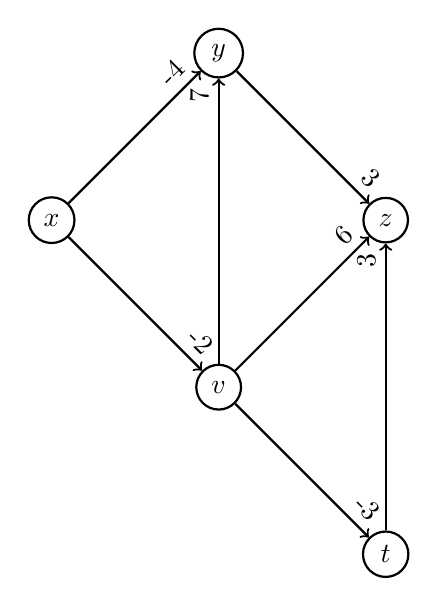
\begin{tikzpicture}[node distance={30mm}, thick, main/.style = {draw, circle}]
    \node[main] (1) {$x$};
    \node[main] (2) [above right of=1] {$y$};
    \node[main] (3) [below right of=1] {$v$}; 
    \node[main] (4) [below right of=3] {$t$};
    \node[main] (5) [above right of=3] {$z$}; 
    \draw[->] (1) -- node[midway, above left, sloped, pos=1] {-4} (2);
    \draw[->] (1) -- node[midway, above left, sloped, pos=1] {-2} (3);
    \draw[->] (2) -- node[midway, above left, sloped, pos=1] {3} (5);
    \draw[->] (3) -- node[midway, above left, sloped, pos=1] {6} (5);
    \draw[->] (3) -- node[midway, above left, sloped, pos=1] {7} (2);
    \draw[->] (3) -- node[midway, above left, sloped, pos=1] {-3} (4);
    \draw[->] (4) -- node[midway, above left, sloped, pos=1] {3} (5);
    \end{tikzpicture}
     
     Observam din desen ca drumul de cost minim dintre nodurile \textit{x} si \textit{z} este urmatorul: \textit{x  $\rightarrow$ v  $\rightarrow$ t  $\rightarrow$ z}, cu costul -2.
     
      Acum daca luam toate costurile arcelor si le adunam cu constanta \textit{c}, \textit{c}
     fiind \textit{$\mid$min(a)$\mid$} adica modulul minimului functiei \textit{a} (stim exact ca \textbf{exista} macar un arc cu cost minim), drumul initial de cost minim \textit{x  $\rightarrow$ v  $\rightarrow$ t  $\rightarrow$ z} va deveni de cost 10 (-2 + (-3) + 3 + 4 + 4 + 4), dar in digraf exista si drumul \textit{x  $\rightarrow$ y  $\rightarrow$ z} care va deveni de cost 7 iar acesta initial era de cost -1 (adica nu era in digraf initial un drum de cost minim). Deci contraexemplul functioneaza si astfel algoritmul nu este valid pentru problema aceasta.
\section*{Exercitiul 4}
    \quad Fie \textit{G=} (\textit{V,E}), un \textit{s $\in$V}, cu o functie de cost \textit{a : A $\rightarrow$ R} astfel incat 
    $$
    a(s,i) = \begin{cases}
        <0  \text{, daca i este vecin cu s} \\
        \geq 0  \text{, altfel}
    \end{cases}
    $$
 
    \quad Fie \textit{s $\rightarrow$ j} un drum de cost minim in care exista un \textit{k $\in$ V, k $\in$N\tiny{G}\large(s)}. Stim ca drumul de cost minim \textit{k $\rightarrow$ j} este un drum de cost minim din corectitudinea algoritmului Dijkstra (orice arc este de cost positiv). (*)
    
    \quad Pentru a demonstra ca drumul \textit{s $\rightarrow$ k} este de cost minim vom alege o constanta \textit{c este $\mid$min(a(s,i))$\mid$ pentru $\forall$i $\in$N\tiny{G}\large(s)} (vom aduce toate arcele la cost positiv). Intrucat doar costurile arcelor care ies din \textit{s} s-au schimbat drumul   \textit{s $\rightarrow$ k} tot ramane acelasi deci algoritmului Dijkstra este corect si pentru drumul \textit{s $\rightarrow$ k}. (**)
    
    \quad Din (*) si (**): Algoritmului Dijkstra este corect astfel drumul \textit{s $\rightarrow$ j pentru $\forall$j $\in$ V} este cel de cost minim.
      
\end{document}